\section{Aufbau}
\label{sec:Aufbau}
Der Aufbau ist in \autoref{fig:Aufbau} dargestellt.
\begin{figure}[H]
    \centering
    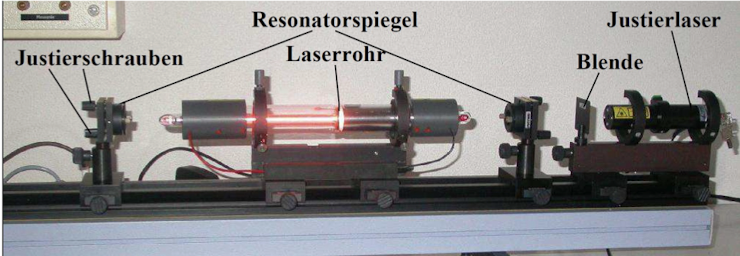
\includegraphics[scale=0.7]{Abbildungen/Aufbau.png}
    \caption{Bild von dem Versuchsaufbau.\cite{V61}}
    \label{fig:Aufbau}
\end{figure}
Dabei besteht dieser aus einer optischen Schiene, auf welcher verschieden Bauteile montiert werden können.
Auf der rechten Seite ist ein Justierlaser, welcher ausgerechnet werden muss. Dafür kann ein Schirm mit Fadenkreuz und eine Beugungsblende
dirket hinter dem Justierlaser und am Ende der optischen Bank positioniert werden. Es ist richtig ausgrechnet, wenn die 
Beugungsringedirekt im Fadenkreuz liegen.\\
Der eigentliche Laser besteht aus einem Laserrohr und zwei hochreflektierenden Spiegeln.
Es gibt verschieden Spiegel, die ausgetauscht werden können. Diese bilden den Laserresonator.
Das Laserrohr ist mit einem Gasgemisch gefüllt und mit Elektroden versehen. dadurch, kann mittels Entladung eine Inversion stattfinden.
Damit einen definierte Polarisationsrichtung gewährleistet ist, befinden sich am Ende der Laserröhre BrewsterFenster.\\
In den Strahlengang können verschieden Komponenten eingefügt werden um die Lasereigenschaften zu vermessen.

\section{Durchführung}
\label{sec:Durchführung}
Im Folgenden wird die Durchführung in die Justage und das Messprogramm unterteilt.

\subsection{Justage des He-Ne-Lasers}
\label{subsec:Justage}
Der Justierlaser wird mit den Beugungsblenden auf die optische Schiene gestellt, wobei die Belnden den maximalen abstand besitzen sollen.
Anschließend muss der Laser so ausgerichtet werden, dass in der Mitte der Beugungsringe die Fadenkreuze liegen.
Danach werden nach und nach die Spiegel und das Laserrohr, wie in \autoref{fig:Aufbau2}.
\begin{figure}[H]
    \centering
    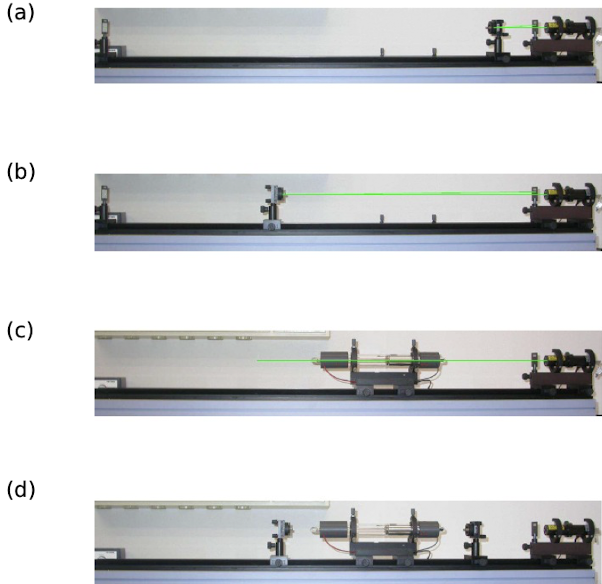
\includegraphics[scale=0.7]{Abbildungen/Aufbau2.png}
    \caption{Bild von dem Versuchsaufbau.\cite{V61}}
    \label{fig:Aufbau2}
\end{figure}
Dabei muss nach jeder Komponente drauf geachtet werden, dass der Rückreflex des Justierlasers wieder auf die Justierblende im Fadenkreuz trifft.
Damit ist die Justierung des Lasers beendet. Es wird der Justierlaser ausgestellt und der Strom der Hochspannung
auf $I = \qty{6.5}{\milli\A}$ eingestellt. Die Lasertätigkeit wird eingestellt, indem an den Justierschrauben der Resonatorspiegel nachjustiert wird.
